%
%
%

\begin{frame}{Autoencoders}

    Autoencoders are a type of neural network that can learn to compress 
    and decompress data, typically used for unsupervised learning tasks.
    
    \begin{figure}[h]
    \centering
    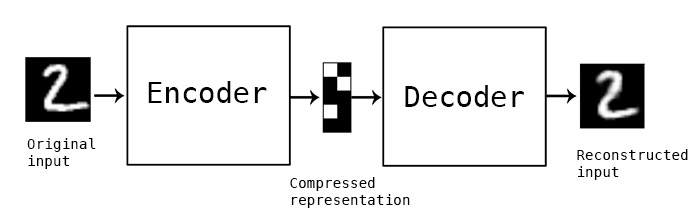
\includegraphics[width=0.8\textwidth]{./images/autoencoders/autoencoder_schema.png}\\
    {\scriptsize 
    \color{col:attribution} 
    Image reproduced from \cite{KerasBlog:BuildingAutoencodersInKeras}}\\
    \end{figure}
    
    \begin{itemize}
    \item The encoder takes in raw input data and compresses it into a smaller, encoded representation.
    \item The decoder takes this encoded representation and tries to reconstruct the original input.
    \item The goal is to minimise the reconstruction error, i.e., make the output as close to the input as possible.
    \item Autoencoders can be used for tasks such as dimensionality reduction, image denoising, and anomaly detection.
    \end{itemize}
    
\end{frame}

%
%
%

\begin{frame}{Types of autoencoders}

    \begin{itemize}
        \item
        Standard Autoencoder: 
        This is the basic type of autoencoder consisting of an encoder 
        network that maps the input to a lower-dimensional latent space, 
        and a decoder network that reconstructs the input from the latent representation.
        \item
        Convolutional Autoencoder: This type of autoencoder uses convolutional 
        layers in the encoder and decoder networks to handle images or other structured data.
        \item
        Variational Autoencoder (VAE): This is a probabilistic generative 
        model that learns a latent representation for input data and generates 
        new samples by sampling from the learned latent space.
        \item
        Denoising Autoencoder: This type of autoencoder is trained to 
        reconstruct the original input from a corrupted or noisy input, 
        making it useful for image or signal denoising.
        \item
        Recurrent Autoencoder: This type of autoencoder is used for
        sequence data such as text, speech, or time-series data.
        \item
        Sparse Autoencoder: This type of autoencoder is trained to 
        learn a sparse representation of the input data by adding a 
        sparsity constraint to the loss function.
        \item
        Adversarial Autoencoder (AAE): This type of autoencoder is a 
        generative model that combines autoencoders with adversarial 
        networks to generate new samples that resemble the input data.
        \item
        Contractive Autoencoder: This type of autoencoder is trained 
        to learn a compressed representation of the input data while 
        preserving its structure by adding a regularisation term to the 
        loss function that penalizes the sensitivity of the output to small changes in the input.
    \end{itemize}

\end{frame}